\section{Results and Discussion}
\label{sec:results}

\subsection{mdHODMDit Applied to the CORIA Dataset} 
\label{sec:results_coria}

The main results reported in this section are build upon the work of Pablo López Salazar that first started the collaboration with CORIA. mdHODMDit described in section~\ref{sec:method_mdhodmd} is applied to extract core physical behaviour of the system in the three cases reported in section~\ref{sec:datasets}. 

\subsubsection{Data Structure and Preprocessing}
\label{sec:coria_preprocessing}

For each case, data is organized in a four dimensional tensor: $\mathcal{T} \in \mathbb{R}^{N_{\mathrm{var}} \times N_x \times N_y \times N_t}$, in which the dimension correspond to variables, the streamwise spatial coordinate $x$, the cross-stream coordinate $y$, and time $t$, respectively.
In order to study the region of physical interest, i.e. the one in which the instability develops and evolves the domain of the streamwise direction is restricted to the range $[0.3, 5.0]$~cm downstream of the splitter plate. This is the near-field flame stabilization region and the initial development of the shear layer. Data was also processed in time discarding the initial transient regime. 
For this kind of data, scaling is important due to the differences in the order of magnitude of the variables considered and the differences between their units of measurement \cite{corrochano2023higher, parente2013principal}. Since there is no universally accepted quantitative criterion to determine which scaling method is most appropriate, the analysis was performed using both auto scaling $x_{i}^{\text{scaled}} = \frac{x_i - \mu_x}{\sigma_x}$ and range scaling $x_{i}^{\text{scaled}} = \frac{x_i - x_{\min}}{x_{\max} - x_{\min}}$. The analysis yielded similar results for both scaling methods, identifying the same main frequencies.
For convenience, frequencies are expressed in units of Strouhal number: 
\begin{equation}
    St = f \cdot \frac{\ell}{U_b},
\label{eq:strouhal}
\end{equation}
where $\ell = 3$~mm is the reference lenght of the mixing layer and  $U_b$ is the bulk speed, respectively $U_b = 21{,}34$, $24{,}29$ e $27{,}14$~m~s$^{-1}$ for cases at 1200~K, 1500~K e 1700~K.

\subsubsection{Parameter Calibration}
\label{sec:coria_params}

The analysis is performed over a grid of Hankel delay parameters
\begin{equation}
    d \in \{10,\, 15,\, 20,\, 25,\, 30,\, 35,\, 40,\, 45\}
    \label{eq:d_values}
\end{equation}
and tolerance values
\begin{equation}
    \varepsilon_{\mathrm{tol}} \in
    \{5\times10^{-3},\, 2\times10^{-2},\, 3\times10^{-2},\, 4\times10^{-2},\,
      5\times10^{-2},\, 7\times10^{-2},\, 1\times10^{-1},\, 2\times10^{-1}\}.
    \label{eq:tol_values}
\end{equation}
The same tolerance $\varepsilon_{\mathrm{tol}}$ governs both the HOSVD truncation (equation~\eqref{eq:hosvd_trunc}) and the amplitude threshold applied to retain DMD modes.




\subsubsection{Frequency--Amplitude Spectra and associated DMD modes}
\label{sec:freq_amplitude}

The frequency--amplitude plots shown in Figures~\ref{fig:spectrum_1200K}, \ref{fig:spectrum_1500K}, and \ref{fig:spectrum_1700K} display, for each temperature case, the normalised DMD mode amplitudes $|\hat{a}_k| / \max_k |\hat{a}_k|$ as a function of Strouhal number $St$. Each marker corresponds to one $(d, \varepsilon_{\mathrm{tol}})$ pair; different colours encode different values of $d$ and different marker styles encode different tolerances. Peaks that persist across all curves can therefore be read off directly as physically robust frequencies. To showcase the coherent structures associated to these freuqencies, temperature is choosen as the rapresentative variable due to the fact that in many cases is a variable of interest for both experimental and theoretical problems. Despite this, coherent structures for every variable can be plotted.

\paragraph{Case 1200~K}
\label{sec:spectrum_1200K}

The spectrum for the 1200~K case, shown in Figure~\ref{fig:spectrum_1200K}, is characterised by a rich distribution of modes spanning a broad Strouhal range up to $St \approx 1.7$. The dominant peak is located at $St \approx 0.42$ and is reproduced consistently across all $(d, \varepsilon_{\mathrm{tol}})$ combinations, confirming its physical robustness. Secondary peaks of significant amplitude are identified at $St \approx 0.84$, $St \approx 1.26$, $St \approx 1.68$. These peaks are approximately integer multiples of the dominant frequency and therefore interpretable as higher harmonics of the fundamental shear-layer instability. 

\FloatBarrier
\begin{figure}[h!]
    \centering
    
\includegraphics[width=\textwidth]{Frequency_amplitude_plot1200.png}
    \caption{Normalised DMD mode amplitudes as a function of Strouhal number for the 1200~K dataset, for $d \in \{35,40,45\}$ and $\varepsilon_{\mathrm{tol}} \in \{5\times10^{-2},\, 7\times10^{-2}\}$.}
    \label{fig:spectrum_1200K}
\end{figure}
\FloatBarrier

The associated modes to the highlighted points in Figure~\ref{fig:spectrum_1200K} are shown in Figure~\ref{fig:modes_1200K}.

\FloatBarrier
\begin{figure}[h!]
    \centering
    \begin{subfigure}[b]{0.48\textwidth}
        \centering
        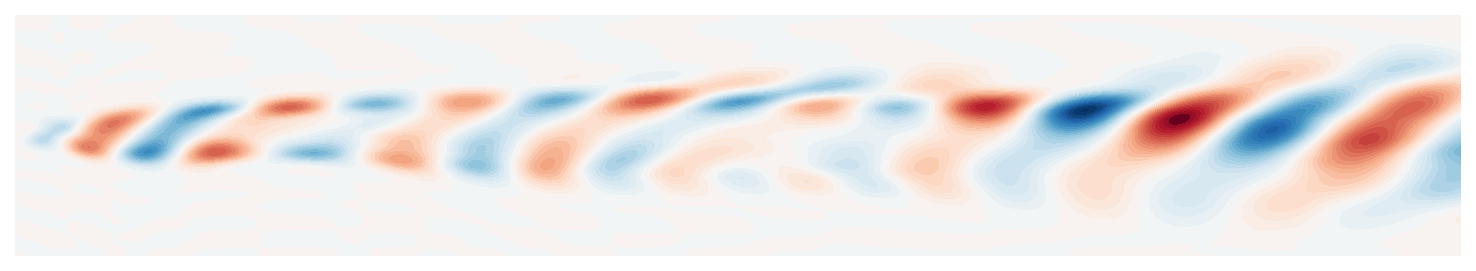
\includegraphics[width=\linewidth]{IMAGES/DMD_MODES_main_freqs_T1200/DMD_mode_St0.42.png}
        \caption{Mode at $St = 0.42$}
        \label{fig:modes_1200K_1}
    \end{subfigure}
    \hfill
    \begin{subfigure}[b]{0.48\textwidth}
        \centering
        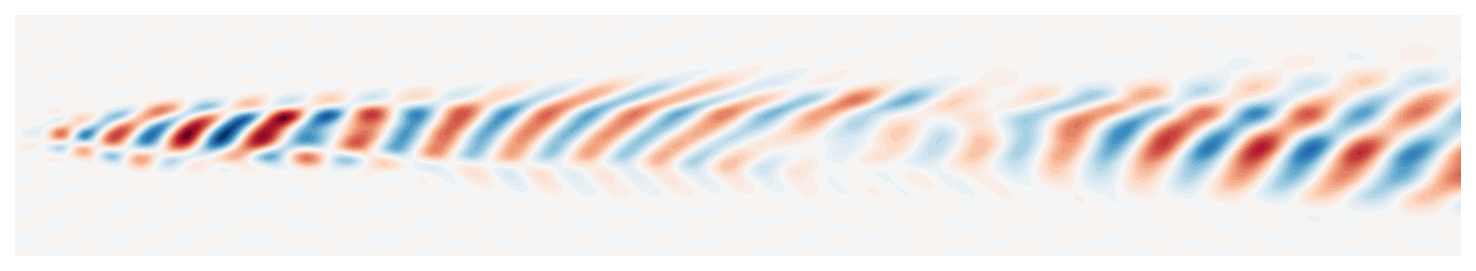
\includegraphics[width=\linewidth]{IMAGES/DMD_MODES_main_freqs_T1200/DMD_mode_St0.84.png}
        \caption{Mode at $St = 0.84$}
        \label{fig:modes_1200K_2}
    \end{subfigure}
    \\[1em]
    \begin{subfigure}[b]{0.48\textwidth}
        \centering
        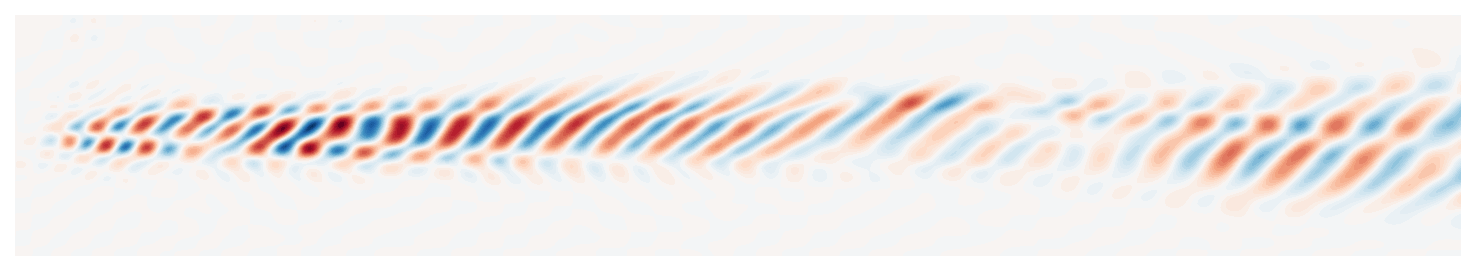
\includegraphics[width=\linewidth]{IMAGES/DMD_MODES_main_freqs_T1200/DMD_mode_St1.26.png}
        \caption{Mode at $St = 1.26$}
        \label{fig:modes_1200K_3}
    \end{subfigure}
    \hfill
    \begin{subfigure}[b]{0.48\textwidth}
        \centering
        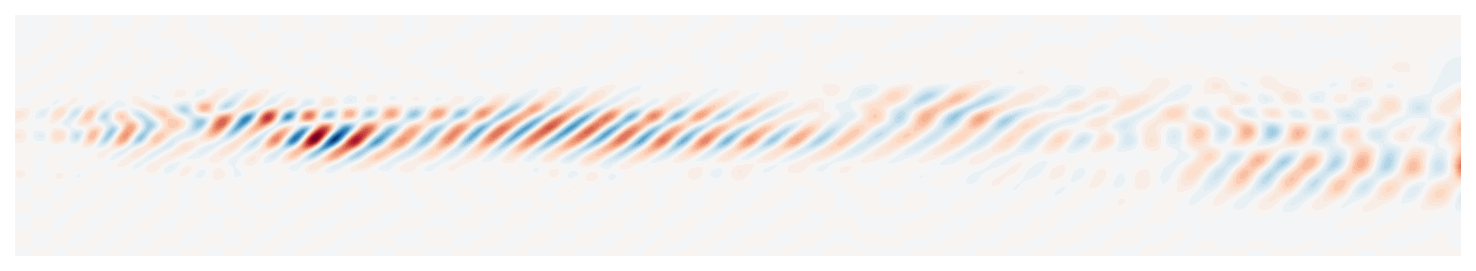
\includegraphics[width=\linewidth]{IMAGES/DMD_MODES_main_freqs_T1200/DMD_mode_St1.68.png}
        \caption{Mode at $St = 1.68$}
        \label{fig:modes_1200K_4}
    \end{subfigure}
    \caption{DMD temperature modes for the 1200~K dataset at the main harmonic frequencies ($St = 0.42$, $0.84$, $1.26$, $1.68$), corresponding to $f$, $2f$, $3f$, and $4f$ respectively.}
    \label{fig:modes_1200K}
\end{figure}
\FloatBarrier


\paragraph{Case 1500~K}
\label{sec:spectrum_1500K}

The 1500~K spectrum, shown in Figure~\ref{fig:spectrum_1500K_combination}, exhibits a structure closely analogous to the 1200~K case, with the dominant peak again located at $St \approx 0.42$. Secondary peaks are found at $St \approx 0.81$, $St \approx 1.22$, and $St \approx 1.47$.  In this case however, the spectrum shows other spectral peaks as highlighted in Figure~\ref{fig:spectrum_1500K_combination} in green. These peaks rapresent the interaction between main frequencies typical of the quasi periodic regime. 
\FloatBarrier
\begin{figure}[h!]
    \centering
    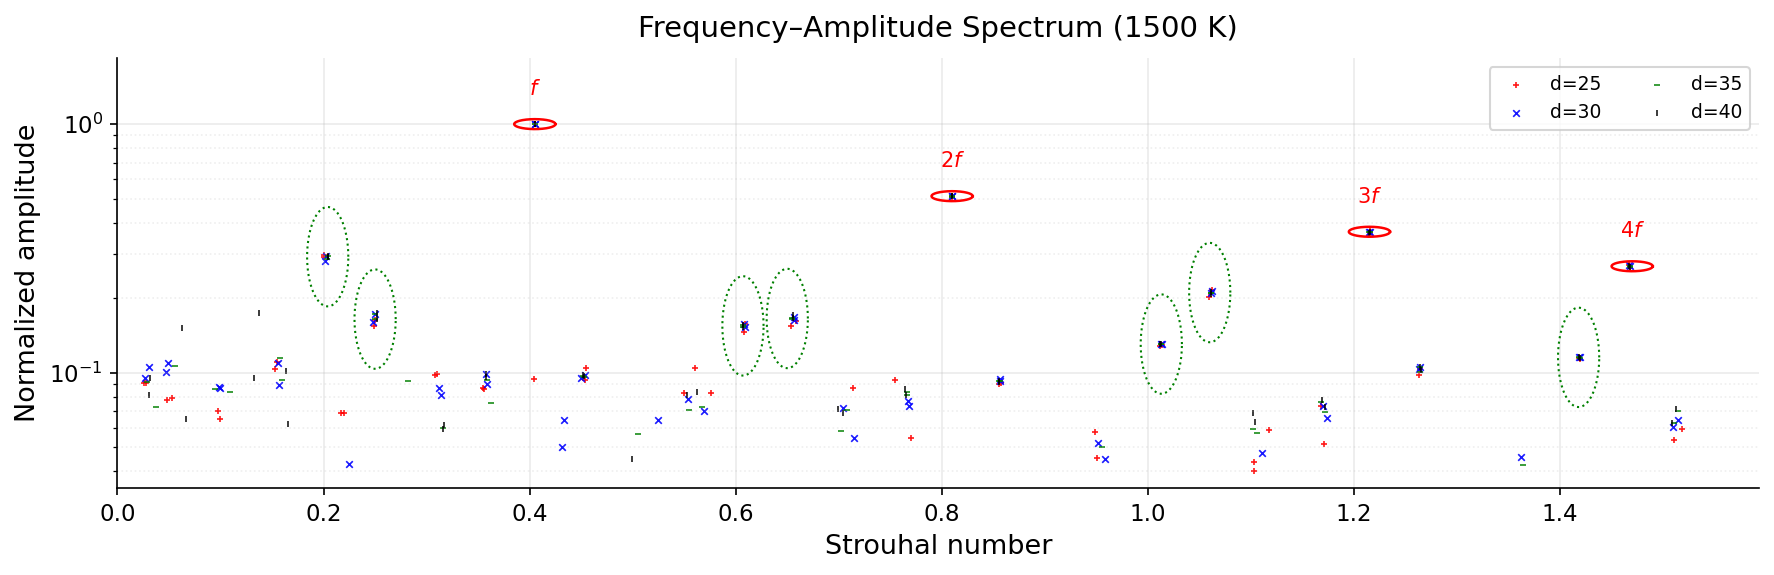
\includegraphics[width=\textwidth]{IMAGES/Spectrum_1500K_d25_30_35_40_tol4e-02_5e-02.png}
    \caption{Normalised DMD mode amplitudes as a function of Strouhal number for the 1500~K dataset, for $d \in \{35,40,45\}$ and $\varepsilon_{\mathrm{tol}} \in \{5\times10^{-2},\, 7\times10^{-2}\}$. Red solid ellipses mark the main harmonic series ($f$, $2f$, $3f$); green dashed ellipses mark the quasi-periodic combination tones ($f_2$, $f+f_2$, $2f+f_2$, $3f+f_2$).}
    \label{fig:spectrum_1500K_combination}
\end{figure}
\FloatBarrier



The associated modes to the main harmonic frequencies circled in red in Figure~\ref{fig:spectrum_1500K_combination} are shown in Figure~\ref{fig:modes_1500K}.

\FloatBarrier
\begin{figure}[h!]
    \centering
    \begin{subfigure}[b]{0.48\textwidth}
        \centering
        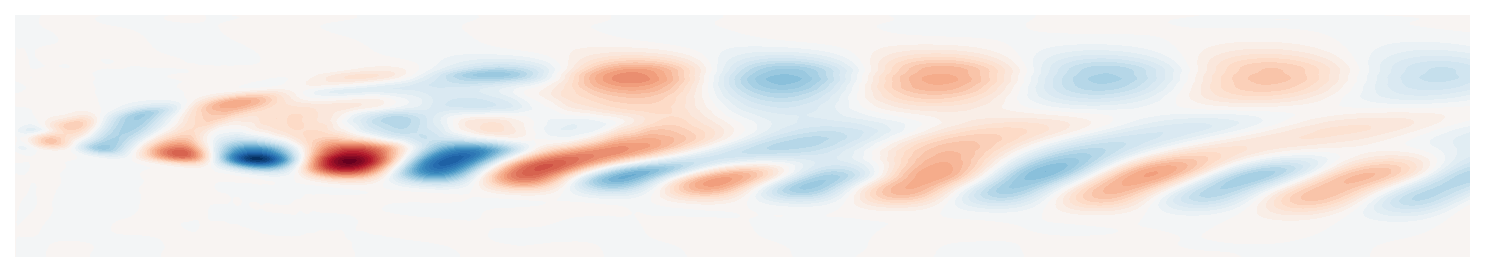
\includegraphics[width=\linewidth]{IMAGES/DMD_MODES_main_freqs_T1500/DMD_mode_St0.41.png}
        \caption{Mode at $St = 0.41$}
        \label{fig:modes_1500K_1}
    \end{subfigure}
    \hfill
    \begin{subfigure}[b]{0.48\textwidth}
        \centering
        
\includegraphics[width=\linewidth]{IMAGES/DMD_MODES_main_freqs_T1500/DMD_mode_St0.81.png}
        \caption{Mode at $St = 0.81$}
        \label{fig:modes_1500K_2}
    \end{subfigure}
    \\[1em]
    \begin{subfigure}[b]{0.48\textwidth}
        \centering
        
\includegraphics[width=\linewidth]{IMAGES/DMD_MODES_main_freqs_T1500/DMD_mode_St1.22.png}
        \caption{Mode at $St = 1.22$}
        \label{fig:modes_1500K_3}
    \end{subfigure}
    \hfill
    \begin{subfigure}[b]{0.48\textwidth}
        \centering
        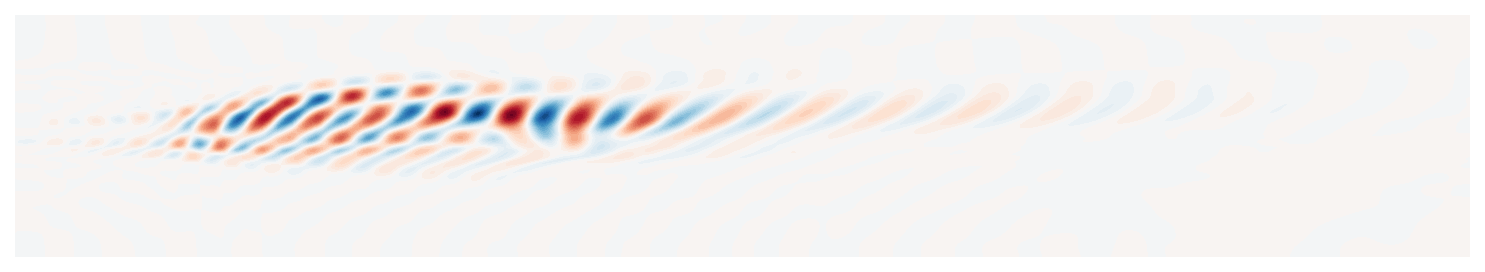
\includegraphics[width=\linewidth]{IMAGES/DMD_MODES_main_freqs_T1500/DMD_mode_St1.47.png}
        \caption{Mode at $St = 1.47$}
        \label{fig:modes_1500K_4}
    \end{subfigure}
    \caption{DMD temperature modes for the 1500~K dataset at the main harmonic frequencies ($St = 0.41$, $0.81$, $1.22$, $1.47$), corresponding to $f$, $2f$, $3f$, and $4f$ respectively.}
    \label{fig:modes_1500K}
\end{figure}
\FloatBarrier

Figure~\ref{fig:comb_modes_1500K} shows the modes associated to the quasi-periodic combination frequencies highlighted in green in Figure~\ref{fig:spectrum_1500K_combination}.
\FloatBarrier
\begin{figure}[h!]
    \centering
    \begin{subfigure}[b]{0.48\textwidth}
        \centering
        
\includegraphics[width=\linewidth]{IMAGES/DMD_MODES_main_freqs_T1500/DMD_mode_St0.20.png}
        \caption{Mode at $St = 0.20$}
        \label{fig:comb_modes_1500K_1}
    \end{subfigure}
    \hfill
    \begin{subfigure}[b]{0.48\textwidth}
        \centering
        
\includegraphics[width=\linewidth]{IMAGES/DMD_MODES_main_freqs_T1500/DMD_mode_St0.61.png}
        \caption{Mode at $St = 0.61$}
        \label{fig:comb_modes_1500K_2}
    \end{subfigure}
    \\[1em]
    \begin{subfigure}[b]{0.48\textwidth}
        \centering
        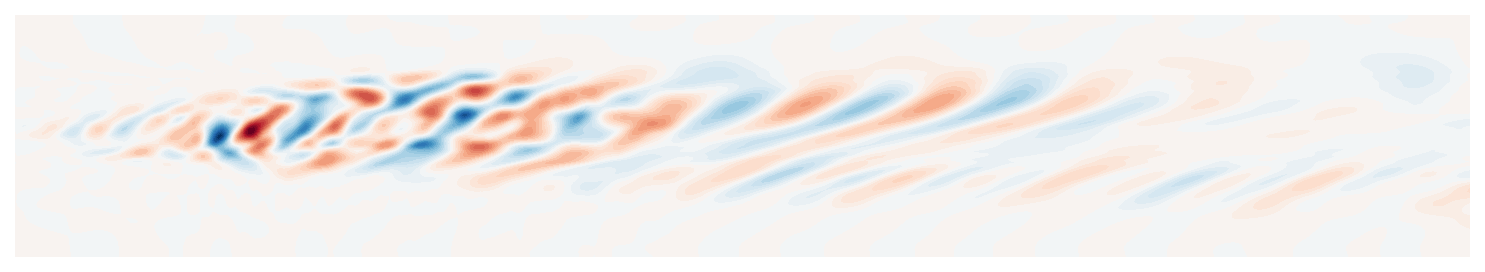
\includegraphics[width=\linewidth]{IMAGES/DMD_MODES_main_freqs_T1500/DMD_mode_St1.01.png}
        \caption{Mode at $St = 1.01$}
        \label{fig:comb_modes_1500K_3}
    \end{subfigure}
    \hfill
    \begin{subfigure}[b]{0.48\textwidth}
        \centering
        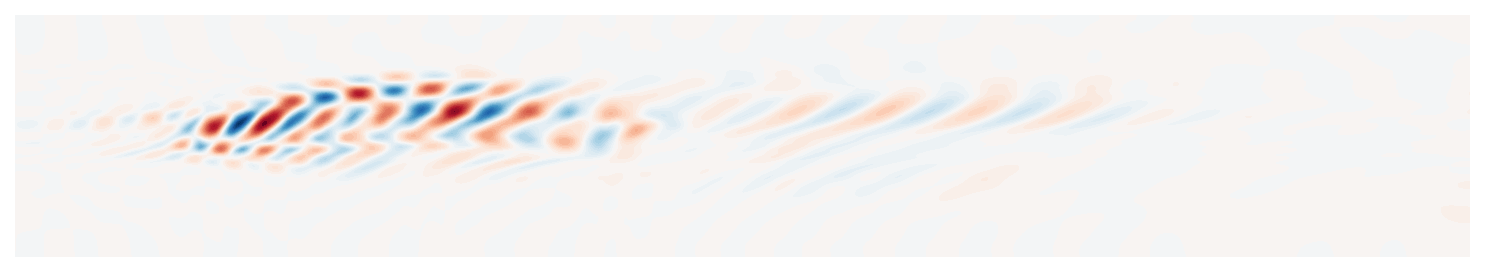
\includegraphics[width=\linewidth]{IMAGES/DMD_MODES_main_freqs_T1500/DMD_mode_St1.42.png}
        \caption{Mode at $St = 1.42$}
        \label{fig:comb_modes_1500K_4}
    \end{subfigure}
    \caption{DMD temperature modes for the 1500~K dataset at the quasi-periodic combination frequencies ($St = 0.20$, $0.61$, $1.01$, $1.42$), highlighted by green ellipses in Figure~\ref{fig:spectrum_1500K_combination}.}
    \label{fig:comb_modes_1500K}
\end{figure}
\FloatBarrier


\paragraph{Case 1700~K}
\label{sec:spectrum_1700K}

The 1700~K case, shown in Figure~\ref{fig:spectrum_1700K}, presents a different spectral structure. The dominant peak remains at $St \approx 0.40$, consistent with the lower-temperature cases, but the overall spectrum is sparser: maximum relevant Strouhal number observed is $St \approx 1.25$ and fewer secondary modes are retained. In addition to the main harmonic series, two low-frequency peaks at $St \approx 0.11$ and $St \approx 0.19$, highlighted in blue in Figure~\ref{fig:spectrum_1700K}, are identified across multiple parameter combinations.

\FloatBarrier
\begin{figure}[h!]
    \centering
    
\includegraphics[width=\textwidth]{Frequency_amplitude_plot1700.png}
    \caption{Normalised DMD mode amplitudes as a function of Strouhal number for the 1700~K dataset, for $d \in \{35,40,45\}$ and $\varepsilon_{\mathrm{tol}} \in \{5\times10^{-2},\, 7\times10^{-2}\}$.}
    \label{fig:spectrum_1700K}
\end{figure}
\FloatBarrier

The associated modes to the highlighted points in Figure~\ref{fig:spectrum_1700K} are shown in Figure~\ref{fig:modes_1700K}.

\FloatBarrier
\begin{figure}[h!]
    \centering
    % Top row: three main harmonics
    \begin{subfigure}[b]{0.32\textwidth}
        \centering
        
\includegraphics[width=\linewidth]{IMAGES/DMD_MODES_main_freqs_T1700/DMD_mode_St0.41.png}
        \caption{Mode at $St = 0.41$}
        \label{fig:modes_1700K_1}
    \end{subfigure}
    \hfill
    \begin{subfigure}[b]{0.32\textwidth}
        \centering
        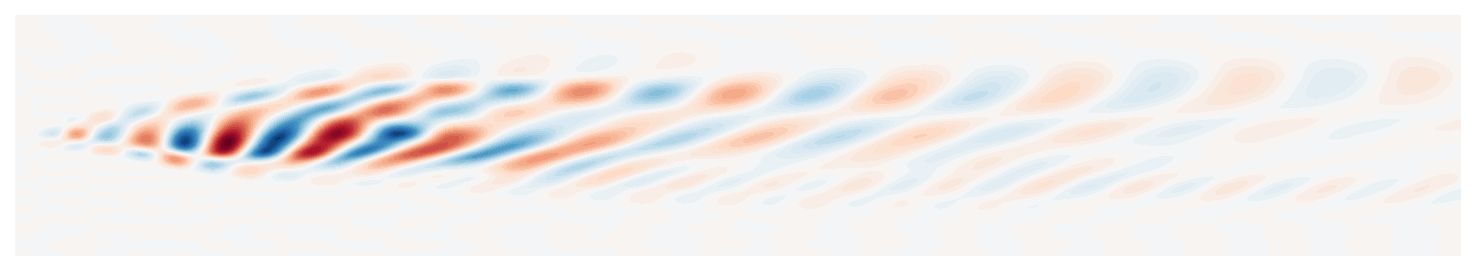
\includegraphics[width=\linewidth]{IMAGES/DMD_MODES_main_freqs_T1700/DMD_mode_St0.82.png}
        \caption{Mode at $St = 0.82$}
        \label{fig:modes_1700K_2}
    \end{subfigure}
    \hfill
    \begin{subfigure}[b]{0.32\textwidth}
        \centering
        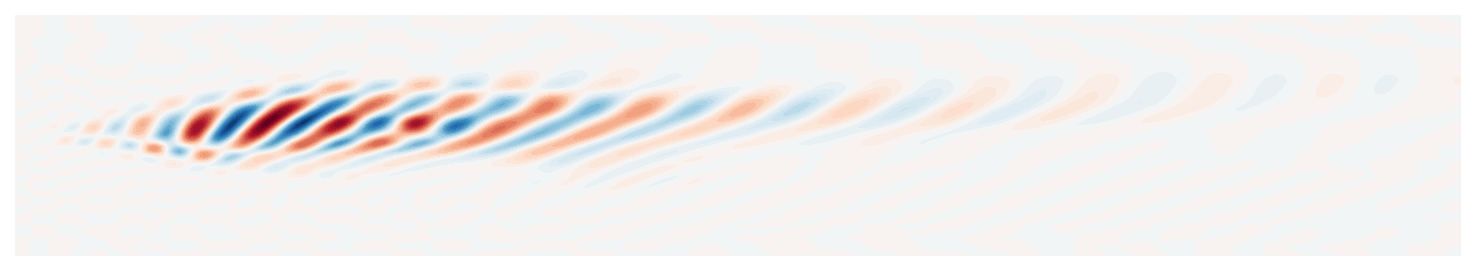
\includegraphics[width=\linewidth]{IMAGES/DMD_MODES_main_freqs_T1700/DMD_mode_St1.23.png}
        \caption{Mode at $St = 1.23$}
        \label{fig:modes_1700K_3}
    \end{subfigure}
    \\[1em]
    % Bottom row: modes at blue-marked frequencies
    \begin{subfigure}[b]{0.48\textwidth}
        \centering
        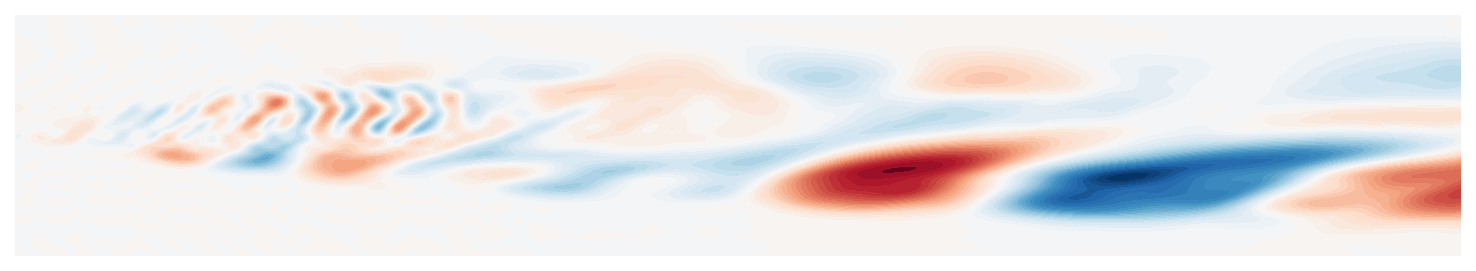
\includegraphics[width=\linewidth]{IMAGES/DMD_MODES_main_freqs_T1700/DMD_mode_St0.11.png}
        \caption{Mode at $St = 0.11$}
        \label{fig:modes_1700K_4}
    \end{subfigure}
    \hfill
    \begin{subfigure}[b]{0.48\textwidth}
        \centering
        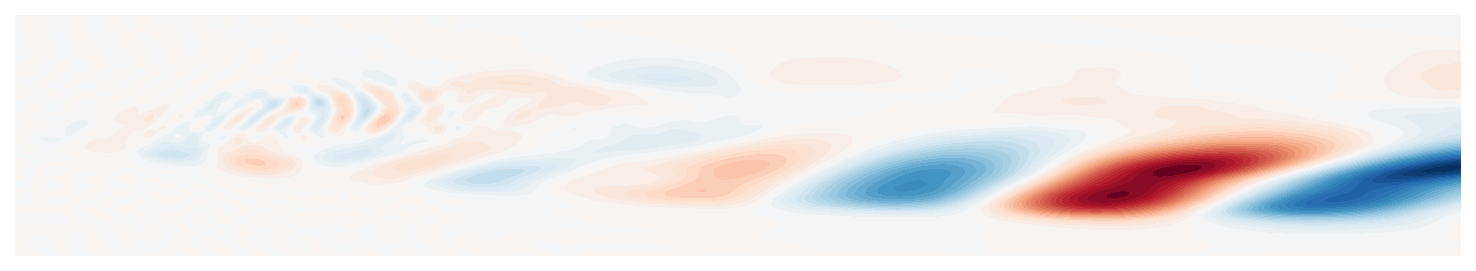
\includegraphics[width=\linewidth]{IMAGES/DMD_MODES_main_freqs_T1700/DMD_mode_St0.19.png}
        \caption{Mode at $St = 0.19$}
        \label{fig:modes_1700K_5}
    \end{subfigure}
    \caption{DMD temperature modes for the 1700~K dataset. Top row: modes at the three main harmonic frequencies ($St = 0.41,\,0.82,\,1.23$). Bottom row: modes at the additional frequencies highlighted in blue in Figure~\ref{fig:spectrum_1700K} ($St = 0.11,\,0.19$).}
    \label{fig:modes_1700K}
\end{figure}
\FloatBarrier

\subsubsection*{Discussion: Spectral and Spatial Evolution Across Preheat Temperatures}

The main focus of this analysis was that of understanding how flow changes in the three cases, rather than investigating the difference in chemical behaviour. Despite this, in practical cases these regimes yield different efficiency-poolutants tradoff, with the lowest temperature case beeing the least efficient and least polluting one and the higher temperature case to have the highest $NO_x$ emission levels and most mixing. 

The first case analyzed, i.e. 1200~K has an harmonic flow with with a dominant peak at $St \approx 0.42$ is accompanied by secondary peaks at approximately integer multiples of this frequency extending up to $St \approx 1.7$. This is the sign of a strongly periodic shear layer instability, and the modes reported in Figure~\ref{fig:modes_1200K} show that the phenomenon develops in the far field. This is reflects downstream convection and roll-up of large-scale vortices that have had space and time to develop along the mixing layer.

On the other hand, at 1700~K, the spectral picture changes substantially. While the dominant frequency is preserved at $St \approx 0.40$, confirming that the primary instability mechanism remains kinematically controlled by the shear between the two inlet streams, the harmonic content is severly reduced, and the overall spectrum is sparser. By observing the modes reported in Figure~\ref{fig:modes_1700K}, one can see that the main instability develops in the near field. This can be explained by the fact that the stronger heat release ties the energetically significant dynamics to the  attachment point.

The 1500~K case contains the transition between the two cases. This is particularly relevant from a physical point of view due to the fact that is a balance between the two regimes. In turn this means that understanding the flow structure might help in designing more efficient combustion processes that suppress $NO_x$ formation.
In this spectrum we can find dominant harmonic structures as in the 1200~K, but additionally the creation of quasi-periodic frequencies highlighted in green in Figure~\ref{fig:spectrum_1500K_combination}. This quasi-periodic spectral content can be interpreted as a signature of the competing dynamics active at this operating point: the primary shear-layer instability is still present, but thermal effects are beginning to modify the nonlinear interactions.
The transient case, i.e. 1500~K has energetically significant DMD modes in both the far field and the near field regions as shown in Figures~\ref{fig:modes_1500K} and \ref{fig:comb_modes_1500K}. In this regime the instabilities are affected by both the far field convective instability and the energy release near the inlet.

Overall, the spectral and spatial analysis consistently shows that increasing preheat temperature progressively anchors the dominant flow dynamics to the near-field region and reduces the coherence of large-scale harmonic structures, with the 1500~K case capturing the transitional regime where both mechanisms are simultaneously active. Further investigation along this research direction, extending the modal analysis to additional operating conditions and coupling it with chemical kinetics data, is expected to provide deeper insight into the mechanisms governing pollutant formation and to support the design of NH$_3$/H$_2$ combustion systems with reduced NO$_x$ emissions.

